\section{ART-MAPPO: Attention-Residual and Trust-Aware MAPPO for Cooperative Swarm Interception}
\label{sec:cooperative_algorithm}

Given the consensus assignment $\mathbf X^{*}$, ART-MAPPO learns cooperative guidance under
the centralized-training--decentralized-execution (CTDE) paradigm. Its information flow is
kept explicit throughout this section: normalized physical observations are encoded by a
task-aware attention-residual backbone, a GRU retains engagement history, trust modulates
training-time exploration, and dual-clip/KL regularization stabilizes the policy update.

\subsection{Task-Aware Attention-Residual Policy Network}
\label{subsec:attention_residual}

Let $\mathbf o_i^{(t)}=[o_i^{(t),1},\ldots,o_i^{(t),n_o}]^{\top}$ denote defender $i$'s
local observation at guidance step $t$. Instead of applying a fully connected layer and then
arbitrarily reshaping mixed features into tokens, we embed each physical channel separately:
\begin{equation}
\label{eq:feature_tokens}
\mathbf H_i^{(0)}=
\begin{bmatrix}
f_1(o_i^{(t),1})^{\top} & \cdots & f_{n_o}(o_i^{(t),n_o})^{\top}
\end{bmatrix}^{\top}
\in\mathbb R^{n_o\times d_e},
\end{equation}
where each $f_r:\mathbb R\rightarrow\mathbb R^{d_e}$ is a learned channel embedding.
Consequently, one token continues to represent one interpretable guidance quantity, such as
LOS rate or time-coordination error.

For attention head $h=1,\ldots,H$, let $d_h=d_e/H$. The complete attention mapping is
\begin{equation}
\label{eq:task_attention}
\begin{aligned}
\mathbf Q_h&=\mathbf H_i^{(0)}\mathbf W_h^Q,\quad
\mathbf K_h=\mathbf H_i^{(0)}\mathbf W_h^K,\quad
\mathbf U_h=\mathbf H_i^{(0)}\mathbf W_h^U,\\
\boldsymbol{\alpha}_h&=\operatorname{softmax}
\left(\frac{\mathbf Q_h\mathbf K_h^{\top}}{\sqrt{d_h}}+\mathbf M_i^{(t)}\right),
\quad \operatorname{head}_h=\boldsymbol{\alpha}_h\mathbf U_h,\\
\mathbf H_{i,\mathrm{att}}&=\mathbf H_i^{(0)}+
\operatorname{Dropout}_p\!\left(
[\operatorname{head}_1\|\cdots\|\operatorname{head}_H]\mathbf W^O\right).
\end{aligned}
\end{equation}
Here, $\mathbf W_h^Q,\mathbf W_h^K,\mathbf W_h^U\in\mathbb R^{d_e\times d_h}$ and
$\mathbf W^O\in\mathbb R^{d_e\times d_e}$, so every matrix dimension is explicit.
$M_{i,rs}^{(t)}=-\infty$ blocks information from an unavailable sensor channel and is zero
otherwise; when all channels are observed, $\mathbf M_i^{(t)}=\mathbf0$. Thus, attention
learns which physical quantities should interact without erasing their channel identities.

The attended tokens are vectorized and projected to $\mathbf h_i^{(1)}\in\mathbb R^d$.
Each of the following $L$ residual blocks is written compactly as
\begin{equation}
\label{eq:residual_block}
\begin{aligned}
\mathbf u_i^{(\ell)}&=\operatorname{ReLU}\!\left(
\operatorname{LN}_1^{(\ell)}
(\mathbf h_i^{(\ell)}\mathbf W_1^{(\ell)}+\mathbf b_1^{(\ell)})\right),\\
\mathcal R_{\ell}(\mathbf h_i^{(\ell)})&=
\operatorname{LN}_2^{(\ell)}\!\left(
\mathbf u_i^{(\ell)}\mathbf W_2^{(\ell)}+\mathbf b_2^{(\ell)}\right),\\
\mathbf h_i^{(\ell+1)}&=\operatorname{ReLU}
\left(\mathbf h_i^{(\ell)}+
\mathcal R_{\ell}(\mathbf h_i^{(\ell)})\right).
\end{aligned}
\end{equation}
The identity shortcut preserves primitive kinematic information and provides a direct gradient
path. It improves optimization conditioning, but no strict nonvanishing-gradient lower bound is
claimed because nonlinear branch derivatives can cancel and ReLU units can be inactive.

A defender-specific GRU state $\mathbf g_i^{(t)}$ summarizes the engagement history, after
which the shared actor samples a bounded continuous guidance action:
\begin{equation}
\label{eq:actor_policy}
\begin{aligned}
\mathbf g_i^{(t)}&=\operatorname{GRU}
(\mathbf h_i^{(L+1)},\mathbf g_i^{(t-1)};\mathbf W_{\mathrm{GRU}}),\\
\mathbf a_i^{(t)}&\sim\pi_{\theta}(\cdot\mid\mathbf o_i^{(t)})
=\mathcal N\!\left(\boldsymbol\mu_{\theta}(\mathbf g_i^{(t)}),
\operatorname{diag}(\boldsymbol\sigma_{\theta}^{2}(\mathbf g_i^{(t)}))\right),\\
\mathbf a_i^{(t)}&=[n_{x_i}^{(t)},n_{y_i}^{(t)},n_{z_i}^{(t)}]^{\top}
\in\mathcal A.
\end{aligned}
\end{equation}
The sampled action is clipped to the three-dimensional load-factor envelope
$\mathcal A=[-0.1,1]\times[-1,1]\times[-1,1]$. The three components regulate speed,
heading, and flight-path angle through Eq.~\eqref{guozai}, respectively.

During training, the centralized critic receives the joint state
\begin{equation}
\label{eq:critic_state}
\mathbf s_t=[\mathbf o_1^{(t)}\|\cdots\|\mathbf o_{N_D}^{(t)}]
\in\mathbb R^{N_Dn_o},\qquad V_{\phi}(\mathbf s_t)\in\mathbb R.
\end{equation}
At deployment, each actor uses only its own observation and recurrent state.

\subsection{Trust-Modulated Tactical Exploration}
\label{subsec:trust_exploration}

Trust is a training-time memory of how reliably a defender performs relative to the recent
swarm baseline; it is not a flight-safety certificate. Let
$G_i^{(k)}=\sum_{t=0}^{H_{\mathrm{ep}}-1}\gamma_{\mathrm{RL}}^t r_i^{(t)}$ be the return
of defender $i$ in episode $k$. Batch statistics and their exponential moving averages are
\begin{equation}
\label{eq:trust_statistics}
\begin{aligned}
\bar G^{(k)}&=\frac{1}{N_D}\sum_{i=1}^{N_D}G_i^{(k)},\qquad
v_G^{(k)}=\frac{1}{N_D}\sum_{i=1}^{N_D}(G_i^{(k)}-\bar G^{(k)})^2,\\
\mu_G&\leftarrow(1-\rho)\mu_G+\rho\bar G^{(k)},\qquad
\sigma_G^2\leftarrow(1-\rho)\sigma_G^2+\rho v_G^{(k)},\\
\widetilde G_i^{(k)}&=\frac{G_i^{(k)}-\mu_G}
{\sqrt{\sigma_G^2+\varepsilon_{\mathrm{num}}}}.
\end{aligned}
\end{equation}
The trust state is then updated by
\begin{equation}
\label{eq:trust_update}
\mathcal T_i^{(k+1)}=(1-\alpha_T)\mathcal T_i^{(k)}
+\alpha_T\sigma(\tau_T\widetilde G_i^{(k)}),
\end{equation}
where $\alpha_T\in(0,1)$ controls memory and $\tau_T>0$ controls sensitivity. Above-baseline
returns increase trust and reduce additional exploration; below-baseline returns do the
opposite.

During training, the action distribution is a trust-dependent mixture
\begin{equation}
\label{eq:exploration_policy}
\begin{aligned}
\pi_i^{\mathrm{mix}}(\mathbf a\mid\mathbf o_i)
&=(1-\beta_i)\pi_{\theta}(\mathbf a\mid\mathbf o_i)
+\beta_i\pi_i^{\mathrm{guide}}(\mathbf a),\\
\pi_i^{\mathrm{guide}}(\mathbf a)&=
\omega_{\mathrm{PN}}\delta(\mathbf a-\mathbf a_{\mathrm{PN}})
+\omega_{\mathrm{pr}}\delta(\mathbf a-\mathbf a_{\mathrm{probe}})\\
&\quad+\omega_{\mathrm{rnd}}\mathcal U(\mathcal A),\\
\beta_i&=1-\mathcal T_i,\qquad
\omega_{\mathrm{PN}}+\omega_{\mathrm{pr}}+\omega_{\mathrm{rnd}}=1.
\end{aligned}
\end{equation}
$\mathbf a_{\mathrm{PN}}$ is the classical PN command clipped to $\mathcal A$.
$\mathbf a_{\mathrm{probe}}$ is a feasible boundary command whose sign is chosen to reduce the
current velocity-to-LOS error; it probes maneuver authority without invoking an undefined
action-value function or intentionally selecting the worst-valued action. The uniform term
maintains residual coverage. At deployment, guided exploration is disabled ($\beta_i=0$), so
the decentralized learned policy supplies the command.

\subsection{Dual-Clip Optimization with Adaptive KL Regularization}
\label{subsec:dual_clip_kl}

For a rollout, generalized advantage estimation is computed from
\begin{equation}
\label{eq:gae}
\begin{aligned}
\delta_t&=r_i^{(t)}+\gamma_{\mathrm{RL}}V_{\phi}(\mathbf s_{t+1})
-V_{\phi}(\mathbf s_t),\\
\widehat A_t&=\sum_{\ell=0}^{H_{\mathrm{ep}}-t-1}
(\gamma_{\mathrm{RL}}\lambda_{\mathrm{GAE}})^{\ell}\delta_{t+\ell}.
\end{aligned}
\end{equation}
Let $\varrho_t(\theta)=\pi_{\theta}(\mathbf a_t\mid\mathbf o_t)/
\pi_{\theta_{\mathrm{old}}}(\mathbf a_t\mid\mathbf o_t)$ denote the importance ratio. The
standard and dual-clipped surrogates are combined in one definition:
\begin{equation}
\label{eq:dual_clip}
\begin{aligned}
\bar\varrho_t&=\operatorname{clip}
(\varrho_t,1-\varepsilon_{\mathrm{PPO}},1+\varepsilon_{\mathrm{PPO}}),\\
L_t^{\mathrm{clip}}&=\min(\varrho_t\widehat A_t,
\bar\varrho_t\widehat A_t),\\
J^{\mathrm{DC}}(\theta)&=\mathbb E_t\!\left[
\begin{cases}
\max(L_t^{\mathrm{clip}},c_{\mathrm{DC}}\widehat A_t),&\widehat A_t<0,\\
L_t^{\mathrm{clip}},&\widehat A_t\geq0,
\end{cases}\right].
\end{aligned}
\end{equation}
For negative-advantage samples, the additional floor prevents an arbitrarily unfavorable
surrogate contribution. It clips the optimization objective; it does not impose a hard
two-sided interval on the realized probability ratio. We use
$c_{\mathrm{DC}}>1+\varepsilon_{\mathrm{PPO}}$.

The empirical policy divergence is
$\widehat D_{\mathrm{KL}}=\mathbb E_t[\log\pi_{\theta_{\mathrm{old}}}
(\mathbf a_t\mid\mathbf o_t)-\log\pi_{\theta}(\mathbf a_t\mid\mathbf o_t)]$. Its penalty
coefficient adapts after epoch $k$ as
\begin{equation}
\label{eq:kl_adaptation}
\beta_{\mathrm{KL}}^{(k+1)}=
\begin{cases}
\min(1.5\beta_{\mathrm{KL}}^{(k)},\beta_{\max}),
&\widehat D_{\mathrm{KL}}>2\delta_{\mathrm{KL}},\\
\max(0.9\beta_{\mathrm{KL}}^{(k)},\beta_{\min}),
&\widehat D_{\mathrm{KL}}<0.5\delta_{\mathrm{KL}},\\
\beta_{\mathrm{KL}}^{(k)},&\text{otherwise}.
\end{cases}
\end{equation}
Thus, excessive policy drift strengthens the next update's penalty, while very small drift
relaxes it. This mechanism controls update speed; any relationship to load-factor smoothness is
validated empirically rather than treated as a structural load bound.

With $\widehat V_t^{\mathrm{targ}}=\widehat A_t+V_{\phi}(\mathbf s_t)$, define
$L_V=B^{-1}\sum_{t=1}^{B}(V_{\phi}(\mathbf s_t)-\widehat V_t^{\mathrm{targ}})^2$ and
$S[\pi_{\theta}]=-\mathbb E_t[\log\pi_{\theta}(\mathbf a_t\mid\mathbf o_t)]$. The complete
training loss is
\begin{equation}
\label{eq:total_loss}
\mathcal L(\theta,\phi)=-J^{\mathrm{DC}}(\theta)
+\beta_{\mathrm{KL}}\widehat D_{\mathrm{KL}}
+c_vL_V-c_eS[\pi_{\theta}].
\end{equation}
The actor minimizes the policy, KL, and entropy terms; the critic minimizes $L_V$. AdamW with
the cosine schedule reported in Table~\ref{table2} performs the updates.

\begin{figure*}[!t]
\centering
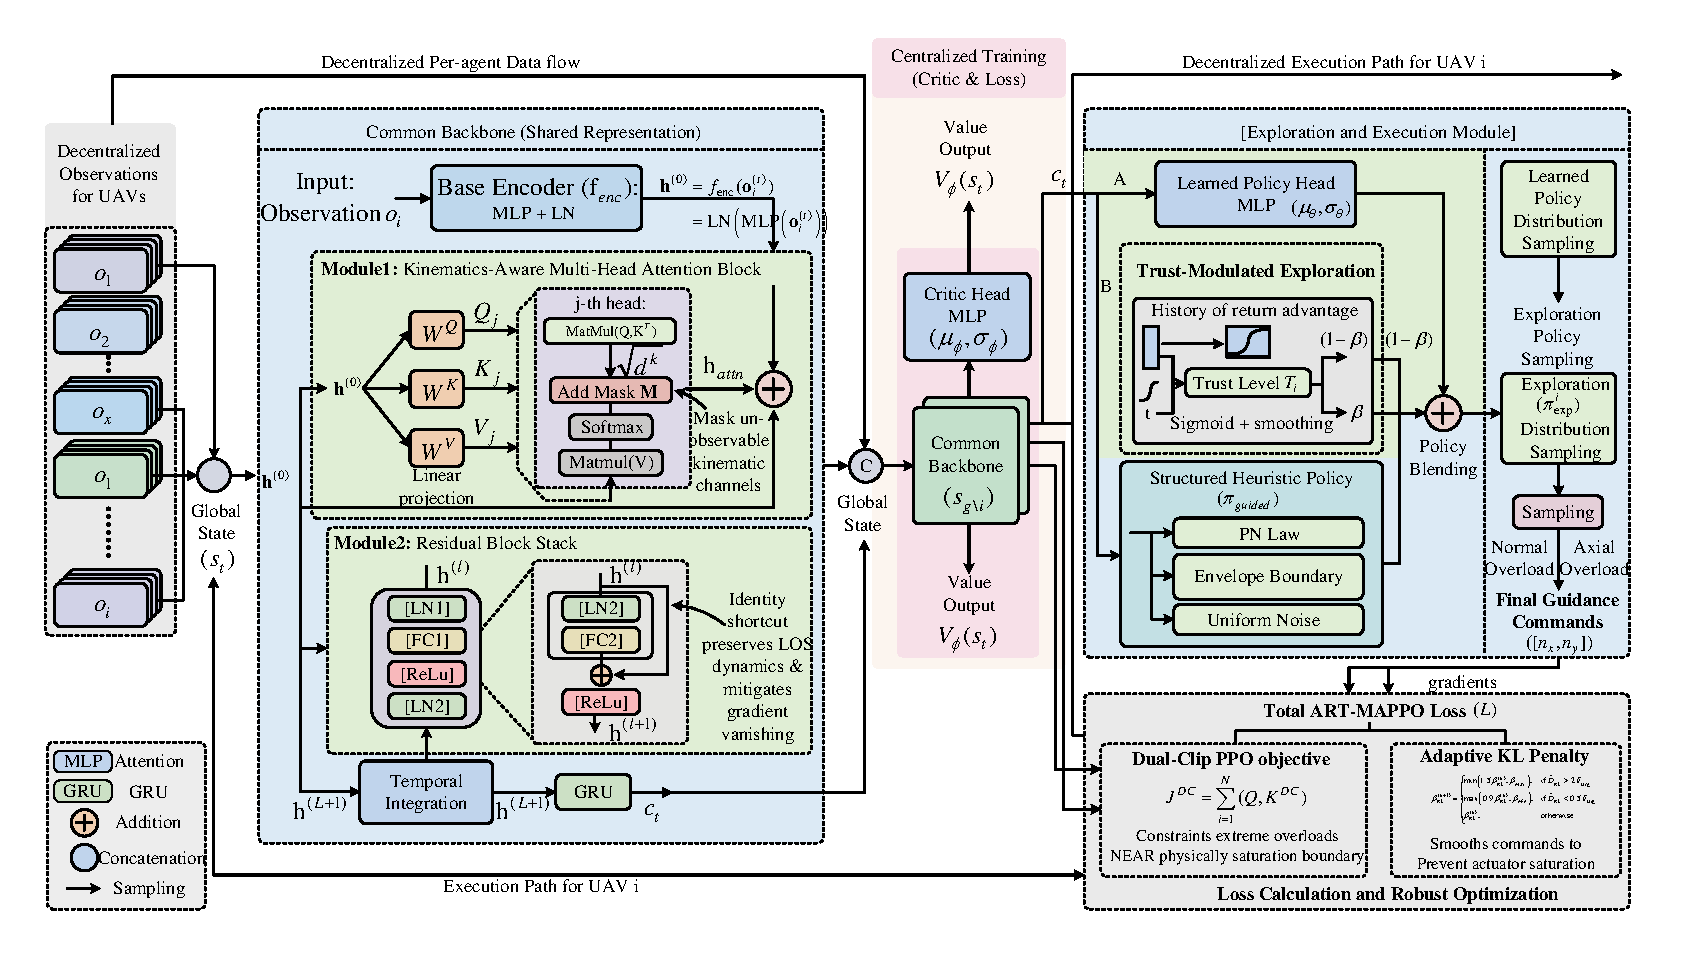
\includegraphics[width=7.0in]{rlsuanfa.pdf}
\caption{ART-MAPPO information flow from physical observations through attention-residual and
recurrent encoding to trust-modulated exploration and regularized actor--critic updates.}
\label{fig:algorithm_flow}
\end{figure*}

\subsection{State Representation and Reward Design}
\label{subsec:state_reward}

The local observation retains relative three-dimensional geometry, cooperative timing, and
the previous applied command. Using fixed physical scales, it is
\begin{equation}
\label{eq:observation_space}
\begin{split}
\mathbf o_i^{(t)}=\operatorname{clip}\bigl([&
d_i/d_{\mathrm{ref}},\ \Delta z_i/z_{\mathrm{ref}},\
\dot d_i/V_{\mathrm{ref}},\ e_{\angle,i}/\pi,\\
&V_i/V_{\mathrm{ref}},\ V_{T(i)}/V_{\mathrm{ref}},\
\theta_i/\pi,\ \gamma_i/\pi,\ \boldsymbol\ell_{iT}^{\top},\\
&(t_{go,i}-\bar t_{go,i})/T_{\mathrm{ref}},\
(t_{go,i}^{\max}-t_{go,i}^{\min})/T_{\mathrm{ref}},\\
&(t_{go,i}-t_{go,i}^{\min})/T_{\mathrm{ref}},\
(\mathbf a_i^{(t-1)})^{\top}]^{\top},-1,1\bigr)
\in\mathbb R^{17}.
\end{split}
\end{equation}
Here, $\Delta z_i$ is the defender--target altitude difference,
$\boldsymbol\ell_{iT}\in\mathbb R^3$ is the LOS unit vector, and
$\widehat{\mathbf v}_i=\mathbf v_i/(\|\mathbf v_i\|_2+\varepsilon_{\mathrm{num}})$ is the
unit velocity direction. Therefore,
$e_{\angle,i}=\arccos[\operatorname{clip}(\widehat{\mathbf v}_i^{\top}
\boldsymbol\ell_{iT},-1,1)]$ is the
three-dimensional velocity-to-LOS angle. The mean, minimum, and maximum time-to-go values are
computed over the cooperative group $\mathcal G_i$. The previous command is available before
the current action is selected and supplies short-term actuator history without violating
causality. Fixed scales $d_{\mathrm{ref}},z_{\mathrm{ref}},V_{\mathrm{ref}}$, and
$T_{\mathrm{ref}}$ make the heterogeneous physical channels comparable.

The reward connects each physical objective to one interpretable component:
\begin{equation}
\label{eq:reward_function}
r_i^{(t)}=\lambda_d r_i^{\mathrm{dist}}
+\lambda_q r_i^{\mathrm{angle}}
+\lambda_h r_i^{\mathrm{hit}}
+\lambda_c r_i^{\mathrm{coord}}
+\lambda_u r_i^{\mathrm{effort}}.
\end{equation}
The components are summarized below to avoid another rapid sequence of five displayed
equations.
\begin{table}[!t]
\centering
\caption{Reward Components and Physical Roles}
\label{tab:reward_components}
\renewcommand{\arraystretch}{1.15}
\footnotesize
\begin{tabular}{@{}p{0.25\linewidth}p{0.67\linewidth}@{}}
\toprule
Component & Definition and role \\
\midrule
$r_i^{\mathrm{dist}}$
& $\exp[-\|\mathbf p_i-\mathbf p_{\mathrm{tgt}}\|/d_{\mathrm{ref}}]$;
bounded dense feedback for closing range.\\
$r_i^{\mathrm{angle}}$
& $-e_{\angle,i}$; penalizes three-dimensional velocity-to-LOS misalignment.\\
$r_i^{\mathrm{hit}}$
& $R_{\mathrm{hit}}\mathbb I[\text{first entry into }d_{\mathrm{kill}}]$;
one-time terminal success reward.\\
$r_i^{\mathrm{coord}}$
& $-|t_{go,i}-|\mathcal G_i|^{-1}\sum_{j\in\mathcal G_i}t_{go,j}|$;
promotes simultaneous arrival.\\
$r_i^{\mathrm{effort}}$
& $-[\|\mathbf a_i^{(t)}\|_2^2+\kappa_{\Delta}
\|\mathbf a_i^{(t)}-\mathbf a_i^{(t-1)}\|_2^2]$;
penalizes all three load channels and their command variation.\\
\bottomrule
\end{tabular}
\end{table}
The environment computes these rewards during training; the critic estimates their discounted
return but does not generate the reward. At deployment, no reward or centralized critic is
required.

\subsection{Sensitivity of Reward Weights and Hyperparameters}
\label{subsec:reward_sensitivity}

The weights $\lambda_d$ and $\lambda_q$ regulate early approach and heading alignment, whereas
$\lambda_h$ and $\lambda_c$ determine the balance between terminal interception and coordinated
arrival. Excessive coordination weight can delay a defender with favorable geometry; excessive
effort weight $\lambda_u$ can suppress the normal-load commands required against a maneuvering
target. We therefore normalize all reward components first, tune hit/coordination weights around
mission success, and then increase the effort term until command peaks and variations satisfy
the desired envelope without degrading interception reliability.

The PPO clipping factor $\varepsilon_{\mathrm{PPO}}$, dual-clip parameter $c_{\mathrm{DC}}$,
target divergence $\delta_{\mathrm{KL}}$, and $\beta_{\mathrm{KL}}$ adaptation determine policy
update conservatism. Smaller clipping/divergence targets improve stability but can slow
adaptation; larger values learn aggressive maneuvers faster but increase return variance.
$\lambda_{\mathrm{GAE}}$ and $c_e$ control the bias--variance and exploration--exploitation
tradeoffs. Their numerical settings and sensitivity tests are reported with the simulation
results rather than expanded into additional equations here.

\begin{algorithm}[!t]
\caption{ART-MAPPO Cooperative Interception Guidance}
\label{alg:artmappo}
\footnotesize
\begin{algorithmic}[1]
\REQUIRE Consensus assignment $\mathbf X^{*}$, environment, episode horizon
$H_{\mathrm{ep}}$, actor $\theta$, critic $\phi$, trust and PPO parameters
\ENSURE Decentralized shared guidance policy $\pi_{\theta}$
\STATE Initialize networks, GRU states $\mathbf g_i$, trust states $\mathcal T_i$, and buffer
$\mathcal D$
\FOR{episode $k=1,2,\ldots$}
    \STATE Reset the scenario and form cooperative groups from $\mathbf X^{*}$
    \FOR{$t=0$ to $H_{\mathrm{ep}}-1$}
        \FOR{each defender $i$}
            \STATE Construct $\mathbf o_i^{(t)}$ using \eqref{eq:observation_space}
            \STATE Encode attention/residual features and update $\mathbf g_i^{(t)}$
            \STATE Sample $\mathbf a_i^{(t)}$ from \eqref{eq:exploration_policy} and clip it
            to $\mathcal A$
        \ENDFOR
        \STATE Execute the joint action and compute \eqref{eq:reward_function}
        \STATE Store the transition in $\mathcal D$
    \ENDFOR
    \STATE Update return statistics and trust using
    \eqref{eq:trust_statistics}--\eqref{eq:trust_update}
    \STATE Estimate $\widehat A_t$ using \eqref{eq:gae}
    \STATE Update actor and critic by minimizing \eqref{eq:total_loss}; adapt
    $\beta_{\mathrm{KL}}$ using \eqref{eq:kl_adaptation}
    \STATE Clear $\mathcal D$
\ENDFOR
\STATE Deploy $\pi_{\theta}$ with local observations, local GRU states, and $\beta_i=0$
\end{algorithmic}
\end{algorithm}
